\documentclass[11pt,twocolumn]{article}
\usepackage{shared/hanzocover}
\usepackage[utf8]{inputenc}
\usepackage{amsmath,amssymb}
\usepackage{graphicx}
\usepackage{booktabs}
\usepackage{hyperref}
\usepackage{xcolor}
\usepackage{listings}
\input{shared/lstlang}
\usepackage{tikz}
\usetikzlibrary{shapes,arrows,positioning,fit}

\definecolor{codegreen}{rgb}{0,0.6,0}
\definecolor{codegray}{rgb}{0.5,0.5,0.5}
\definecolor{codepurple}{rgb}{0.58,0,0.82}
\definecolor{backcolour}{rgb}{0.95,0.95,0.92}

\lstdefinestyle{mystyle}{
    backgroundcolor=\color{backcolour},
    commentstyle=\color{codegreen},
    keywordstyle=\color{codepurple},
    numberstyle=\tiny\color{codegray},
    stringstyle=\color{codegreen},
    basicstyle=\ttfamily\footnotesize,
    breakatwhitespace=false,
    breaklines=true,
    captionpos=b,
    keepspaces=true,
    numbers=left,
    numbersep=5pt,
    showspaces=false,
    showstringspaces=false,
    showtabs=false,
    tabsize=2
}
\lstset{style=mystyle}

\title{Hanzo PubSub: NATS-Based Event Streaming for Microservice Communication}
\author{Antje Worring, Zach Kelling\thanks{zach@hanzo.ai} \\ \textit{Hanzo Industries} \\ \texttt{research@hanzo.ai}}
\date{January 2022}

\begin{document}

\hanzocoverpage

\begin{abstract}
We present Hanzo PubSub, an event streaming platform built on NATS and JetStream that provides at-least-once delivery, dead letter queues, schema validation, and multi-tenant topic isolation for the Hanzo microservice ecosystem. PubSub replaces direct HTTP calls between services with asynchronous event streams, reducing coupling and enabling event-driven architectures. The system processes 120,000 events per second with a median publish-to-consume latency of 1.8ms. Key design decisions include: (1) tenant-prefixed subject namespaces for isolation without separate NATS clusters, (2) CloudEvents~\cite{cloudevents2019} as the canonical event envelope for cross-service interoperability, and (3) automatic dead letter routing with configurable retry policies. We describe the event schema design, the delivery guarantee implementation, and the operational patterns for managing event streams in a multi-tenant platform.
\end{abstract}

\section{Introduction}

Microservice architectures require reliable inter-service communication. Synchronous HTTP calls create tight coupling: the caller must know the callee's address, handle its failures, and wait for its response. Event-driven communication decouples services temporally and spatially---producers emit events without knowing which consumers will process them.

Hanzo PubSub provides the event infrastructure for 60+ microservices in the Hanzo platform. Built on NATS~\cite{nats2016} with JetStream persistence, PubSub combines the performance of in-memory pub/sub (microsecond latency for ephemeral events) with the durability of stream storage (at-least-once delivery for critical events).

\paragraph{Contributions.}
\begin{itemize}
    \item A multi-tenant subject namespace design using NATS account isolation and subject prefixing.
    \item CloudEvents-based event envelopes with JSON Schema validation at publish time.
    \item Configurable retry policies with exponential backoff and automatic dead letter routing.
    \item A consumer group abstraction supporting competing consumers, fan-out, and exactly-once processing via idempotency keys.
\end{itemize}

\section{Architecture}

\subsection{System Design}

\begin{figure}[t]
\centering
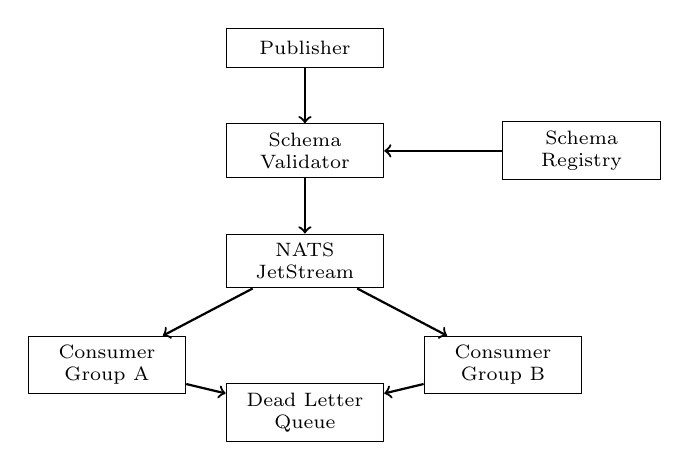
\begin{tikzpicture}[
    node distance=0.7cm,
    box/.style={rectangle, draw, minimum width=2cm, minimum height=0.5cm, align=center, font=\scriptsize},
    arrow/.style={->, thick}
]
\node[box] (pub) {Publisher};
\node[box, below=of pub] (validate) {Schema\\Validator};
\node[box, below=of validate] (nats) {NATS\\JetStream};
\node[box, below left=0.6cm and 0.5cm of nats] (c1) {Consumer\\Group A};
\node[box, below right=0.6cm and 0.5cm of nats] (c2) {Consumer\\Group B};
\node[box, below=1.2cm of nats] (dlq) {Dead Letter\\Queue};
\node[box, right=1.5cm of validate] (registry) {Schema\\Registry};

\draw[arrow] (pub) -- (validate);
\draw[arrow] (validate) -- (nats);
\draw[arrow] (nats) -- (c1);
\draw[arrow] (nats) -- (c2);
\draw[arrow] (c1) -- (dlq);
\draw[arrow] (c2) -- (dlq);
\draw[arrow] (registry) -- (validate);
\end{tikzpicture}
\caption{PubSub event flow with schema validation and dead letter routing.}
\label{fig:pubsub}
\end{figure}

Events flow through a validated pipeline (Figure~\ref{fig:pubsub}): publishers submit events to the schema validator, which checks the event against the registered schema before forwarding to NATS JetStream. Consumer groups receive events with at-least-once delivery. Failed events are routed to dead letter queues after exhausting retry attempts.

\subsection{Event Envelope}

All events use the CloudEvents specification:

\begin{lstlisting}[language=JSON]
{
  "specversion": "1.0",
  "type": "com.hanzo.order.created",
  "source": "/services/commerce",
  "id": "evt_a1b2c3d4",
  "time": "2022-01-15T12:00:00Z",
  "datacontenttype": "application/json",
  "data": {
    "orderId": "ord_xyz",
    "amount": 9999,
    "currency": "USD"
  },
  "hanzoorgid": "org_x7y8z9"
}
\end{lstlisting}

The \texttt{hanzoorgid} extension attribute enables tenant-scoped event routing.

\subsection{Subject Namespace}

NATS subjects follow a hierarchical naming convention:

\begin{verbatim}
{tenant}.{domain}.{entity}.{action}
\end{verbatim}

Examples: \texttt{org\_abc.commerce.order.created}, \texttt{org\_abc.auth.user.login}. Tenant prefixing ensures that consumers in one organization cannot subscribe to another organization's events.

\section{Key Features}

\subsection{Delivery Guarantees}

PubSub supports three delivery modes:

\paragraph{At-Most-Once.} Core NATS pub/sub without JetStream. Used for ephemeral events (metrics, heartbeats) where loss is acceptable. Latency: $<$0.1ms.

\paragraph{At-Least-Once.} JetStream with explicit acknowledgment. Unacknowledged messages are redelivered after a configurable timeout (default: 30s). Used for most business events.

\paragraph{Effectively-Once.} At-least-once delivery combined with consumer-side idempotency checking. The consumer stores processed event IDs in Valkey with a 24-hour TTL.

\subsection{Retry and Dead Letter}

Failed event processing triggers exponential backoff retries:

\begin{equation}
    t_{\text{retry}}(n) = \min(t_0 \cdot 2^n, t_{\max})
\end{equation}

where $t_0 = 1$s, $t_{\max} = 300$s, and the maximum retry count defaults to 5. After exhausting retries, events are published to a dead letter subject (\texttt{\_dlq.{original\_subject}}) for manual investigation or automated recovery.

\subsection{Consumer Groups}

Consumer groups implement competing consumer patterns:

\begin{lstlisting}[language=Go]
sub, _ := js.QueueSubscribe(
    "org_abc.commerce.order.created",
    "fulfillment-workers",
    func(msg *nats.Msg) {
        if err := processOrder(msg); err != nil {
            msg.Nak()  // trigger retry
            return
        }
        msg.Ack()
    },
    nats.Durable("fulfillment"),
    nats.MaxDeliver(5),
    nats.AckWait(30*time.Second),
)
\end{lstlisting}

Within a consumer group, each message is delivered to exactly one consumer. Multiple consumer groups on the same subject each receive every message (fan-out).

\subsection{Schema Registry}

Event schemas are registered in a central registry:

\begin{lstlisting}[language=JSON]
{
  "type": "com.hanzo.order.created",
  "version": 3,
  "schema": {
    "type": "object",
    "required": ["orderId", "amount"],
    "properties": {
      "orderId": {"type": "string"},
      "amount": {"type": "integer", "minimum": 0},
      "currency": {"type": "string", "enum":
        ["USD","EUR","GBP"]}
    }
  }
}
\end{lstlisting}

Schema validation at publish time prevents malformed events from entering the stream. Schema evolution follows a compatibility policy: new fields can be added (backward compatible), required fields cannot be removed (forward compatible).

\section{Implementation}

PubSub is deployed as a 3-node NATS cluster with JetStream enabled. The schema validator and dead letter processor are sidecar containers injected into publisher pods. The Go client library (3,000 lines) wraps the NATS client with schema validation, CloudEvents serialization, and retry logic.

\begin{table}[h]
\centering
\caption{Event processing performance.}
\label{tab:pubsub-perf}
\begin{tabular}{lrr}
\toprule
\textbf{Mode} & \textbf{Latency p50 (ms)} & \textbf{Throughput (evt/s)} \\
\midrule
At-most-once & 0.08 & 850,000 \\
At-least-once & 1.8 & 120,000 \\
Effectively-once & 2.4 & 95,000 \\
\bottomrule
\end{tabular}
\end{table}

\section{Security}

\paragraph{Authentication.} NATS connections require TLS client certificates issued by the Hanzo internal CA. Service identities are extracted from the certificate CN.

\paragraph{Authorization.} NATS account-level permissions restrict which subjects each service can publish to and subscribe from. A service can only publish events in its own domain and subscribe to events it has declared a dependency on.

\paragraph{Encryption.} All inter-node and client-node communication uses TLS~1.3. JetStream storage is encrypted at rest using the filesystem encryption layer.

\paragraph{Audit.} Event metadata (type, source, tenant, timestamp) is indexed in the observability stack. Event payloads containing sensitive data are encrypted at the application level before publishing.

\section{Conclusion}

Hanzo PubSub provides reliable, multi-tenant event streaming that decouples microservice communication while maintaining delivery guarantees. The CloudEvents-based envelope and schema registry ensure interoperability and data quality. Dead letter queues and configurable retry policies handle transient failures automatically. The NATS foundation provides microsecond latency for ephemeral events and millisecond latency with JetStream persistence for durable events.

\bibliographystyle{plain}
\begin{thebibliography}{10}

\bibitem{nats2016}
Synadia Communications. NATS: Cloud Native Messaging System. 2016.

\bibitem{cloudevents2019}
CNCF. CloudEvents: A specification for describing event data in a common way. 2019.

\bibitem{kreps2011}
J. Kreps et al. Kafka: a Distributed Messaging System for Log Processing. NetDB, 2011.

\bibitem{eventdriven2017}
B. Stopford. Designing Event-Driven Systems. O'Reilly, 2018.

\end{thebibliography}

\end{document}
